\chapter{High Peclet Mixing}\label{app:dsm}

% \begin{figure}
    % \centering
    % \input{app_dsm/plots/c_pdfs_time_D.tex}
    % \caption{
    	% The diffuselet method in turbulence, influence of $D$. Parameters: $\mathit{Re}_\lambda = 418$, $s_0 = 10^{-1} \Kolmogorov$, $ds_0 = \left( 10^{-1} \Kolmogorov \right)^2$.
    % }
% \end{figure}
% 
% \begin{figure}
    % \centering
    % \input{app_dsm/plots/c_pdfs_time_s0.tex}
    % \caption{
    	% The diffuselet method in turbulence, influence of $s_0$. Parameters: $\mathit{Re}_\lambda = 418$, $D = 10^{-1} \nu$, $ds_0 = \left( 10^{-1} \Kolmogorov \right)^2$.
    % }
% \end{figure}
% 
% \begin{figure}
    % \centering
    % \input{app_dsm/plots/c_pdfs_time_ds0.tex}
    % \caption{
    	% The diffuselet method in turbulence, influence of $ds_0$. Parameters: $\mathit{Re}_\lambda = 418$, $s_0 = 10^{-1} \Kolmogorov$, $D = 10^{-1} \nu$.
    % }
% \end{figure}
% 
% \begin{figure}
    % \centering
    % \input{app_dsm/plots/time_std_c_D.tex}
    % \caption{
    	% Average (left) and standard deviation (right) of the concentration as a function of time for various diffusion coefficients $D$. Parameters: $\mathit{Re}_\lambda = 418$, $s_0 = 10^{-1} \Kolmogorov$, $ds_0 = (10^{-1} \Kolmogorov)^2$.
    % }
% \end{figure}
% 
% \begin{figure}
    % \centering
    % \input{app_dsm/plots/time_std_c_s0.tex}
    % \caption{
    	% Average (left) and standard deviation (right) of the concentration as a function of time for various initial surface element thickness $s_0$. Parameters: $\mathit{Re}_\lambda = 418$, $D = 10^{-1} \nu$, $ds_0 = (10^{-1} \Kolmogorov)^2$.
    % }
% \end{figure}
% 
% \begin{figure}
    % \centering
    % \input{app_dsm/plots/time_std_c_ds0.tex}
    % \caption{
    	% Average (left) and standard deviation (right) of the concentration as a function of time for various initial surface element surface $ds_0$. Parameters: $\mathit{Re}_\lambda = 418$, $s_0 = 10^{-1} \Kolmogorov$, $D = 10^{-1} \nu$.
    % }
% \end{figure}

\section{Diffuselet Method}

We use the diffuselet method to simulate mixing in a fully turbulent flow ($\mathit{Re}_{\lambda} = 418$).
The resulting statistics are showed in Fig.~\ref{fig:diffuselet_theory_check} for various times.
\begin{figure}
    \centering
    % Reynolds
\begin{tikzpicture}
	\begin{groupplot}[
			group style={
				group size=2 by 2,
				%y descriptions at=edge left,
				%x descriptions at=edge bottom,
				horizontal sep=0.14\linewidth,
				%vertical sep=0.02\linewidth,
			},
			% size
			width=0.48\textwidth,
			% legend
			legend columns=4,
			legend cell align=left,
			legend style={draw=none, fill=none, at={(0.5, 1.1)}, anchor=south},
		]
	% \nextgroupplot[
		% % y
		% ylabel={$p(C = c)$},
		% ymin=1e-9,
		% ymax=1e-6,
		% ymode=log,
		% % x
		% xlabel=$c$,
		% xmin=0,
		% xmax=1,
		% % layers
		% set layers,
		% % legend
		% legend columns=-1,
		% legend cell align=left,
		% legend style={draw=none, fill=none, at={(1.0, 1.1)}, anchor=south},
	% ]
		% \addlegendimage{empty legend}\addlegendentry{$t = ~$}
		% \node[anchor=north west] at (axis cs:0,1e-6) {\textbf{(a)}};
		% % plot
		% \addplot
		% [
		% color=ColorSurf!00!ColorDuration,
		% opacity=1.0,
		% only marks,%solid,
		% %mark repeat=4,
		% mark=star
		% ]
		% table[
			% x expr={\thisrowno{0}},
			% y expr={\thisrowno{1}},
			% col sep=comma,
			% comment chars=\#,
			% unbounded coords=discard,
			% restrict expr to domain={\thisrowno{0}}{0.001:9.009},
		% ]{app_dsm/data/diffuselet/re_lambda_418/tracer__time_0o016__sc_100o0__c_pdf.csv};
		% \addlegendentry{$0.38 \KolmogorovTimeScale$ \quad}
		% % plot
		% \addplot
		% [
		% color=ColorSurf!17!ColorDuration,
		% opacity=1.0,
		% only marks,%solid,
		% %mark repeat=4,
		% mark=*
		% ]
		% table[
			% x expr={\thisrowno{0}},
			% y expr={\thisrowno{1}},
			% col sep=comma,
			% comment chars=\#,
			% unbounded coords=discard,
			% restrict expr to domain={\thisrowno{0}}{0.001:9.009},
		% ]{app_dsm/data/diffuselet/re_lambda_418/tracer__time_0o032__sc_100o0__c_pdf.csv};
		% \addlegendentry{$0.75 \KolmogorovTimeScale$ \quad}
		% % plot
		% \addplot
		% [
		% color=ColorSurf!33!ColorDuration,
		% opacity=1.0,
		% only marks,%solid,
		% %mark repeat=4,
		% mark=o
		% ]
		% table[
			% x expr={\thisrowno{0}},
			% y expr={\thisrowno{1}},
			% col sep=comma,
			% comment chars=\#,
			% unbounded coords=discard,
			% restrict expr to domain={\thisrowno{0}}{0.001:9.009},
		% ]{app_dsm/data/diffuselet/re_lambda_418/tracer__time_0o064__sc_100o0__c_pdf.csv};
		% \addlegendentry{$1.5 \KolmogorovTimeScale$ \quad}
		% % plot
		% \addplot
		% [
		% color=ColorSurf!50!ColorDuration,
		% opacity=1.0,
		% only marks,%solid,
		% %mark repeat=4,
		% mark=pentagon*
		% ]
		% table[
			% x expr={\thisrowno{0}},
			% y expr={\thisrowno{1}},
			% col sep=comma,
			% comment chars=\#,
			% unbounded coords=discard,
			% restrict expr to domain={\thisrowno{0}}{0.001:9.009},
		% ]{app_dsm/data/diffuselet/re_lambda_418/tracer__time_0o128__sc_100o0__c_pdf.csv};
		% \addlegendentry{$3 \KolmogorovTimeScale$ \quad}
		% % plot
		% \addplot
		% [
		% color=ColorSurf!67!ColorDuration,
		% opacity=1.0,
		% only marks,%solid,
		% %mark repeat=4,
		% mark=pentagon
		% ]
		% table[
			% x expr={\thisrowno{0}},
			% y expr={\thisrowno{1}},
			% col sep=comma,
			% comment chars=\#,
			% unbounded coords=discard,
			% restrict expr to domain={\thisrowno{0}}{0.001:9.009},
		% ]{app_dsm/data/diffuselet/re_lambda_418/tracer__time_0o256__sc_100o0__c_pdf.csv};
		% \addlegendentry{$6 \KolmogorovTimeScale$ \quad}
		% % plot
		% \addplot
		% [
		% color=ColorSurf!83!ColorDuration,
		% opacity=1.0,
		% only marks,%solid,
		% %mark repeat=4,
		% mark=square*
		% ]
		% table[
			% x expr={\thisrowno{0}},
			% y expr={\thisrowno{1}},
			% col sep=comma,
			% comment chars=\#,
			% unbounded coords=discard,
			% restrict expr to domain={\thisrowno{0}}{0.001:9.009},
		% ]{app_dsm/data/diffuselet/re_lambda_418/tracer__time_0o512__sc_100o0__c_pdf.csv};
		% \addlegendentry{$12 \KolmogorovTimeScale$ \quad}
		% % plot
		% \addplot
		% [
		% color=ColorSurf!100!ColorDuration,
		% opacity=1.0,
		% only marks,%solid,
		% %mark repeat=4,
		% mark=square
		% ]
		% table[
			% x expr={\thisrowno{0}},
			% y expr={\thisrowno{1}},
			% col sep=comma,
			% comment chars=\#,
			% unbounded coords=discard,
			% restrict expr to domain={\thisrowno{0}}{0.001:9.009},
		% ]{app_dsm/data/diffuselet/re_lambda_418/tracer__time_1o024__sc_100o0__c_pdf.csv};
		% \addlegendentry{$24 \KolmogorovTimeScale$ \quad}


	\nextgroupplot[
		% y
		ylabel={$p(\log \rho)$},
		ymin=1e-4,
		ymax=1e1,
		ymode=log,
		% x
		xlabel=$\log \rho$,
		xmin=-5,
		xmax=50,
		%xtick={-4.605170185988091, 23.025850929940457, 46.051701859880914, 59.86721241784519},
		%xticklabels={$10^{-2}$, $10^{10}$, $10^{20}$, $10^{26}$},
		% layers
		set layers,
	]
		\node[anchor=north west] at (axis cs:-5,1e1) {\scriptsize \textbf{(a)}: $\mathit{Re}_{\lambda} = 25$, $\overline{\lambda} \KolmogorovTimeScale = 0.16$, $V = 0.17 ~ t / \KolmogorovTimeScale$};
		\addlegendimage{empty legend}\addlegendentry{$t \approx ~$}
		% plot
		\addplot
		[
		color=ColorSurf!00!ColorDuration,
		opacity=1.0,
		only marks,%solid,
		mark repeat=10,
		mark=star
		]
		table[
			x expr={\thisrowno{0}},
			y expr={\thisrowno{1}},
			col sep=comma,
			comment chars=\#,
			unbounded coords=discard,
		]{app_dsm/data/diffuselet/re_lambda_25/tracer__time_0o128__log_rho_pdf.csv};
		\addlegendentry{$2 \KolmogorovTimeScale$ \quad}
		\def\modlambda{2.6}
		\def\modtvar{1.0}
		\def\modvar{2.8}
		\def\modt{0.128}
		\addplot
		[
		color=ColorSurf!00!ColorDuration,
		opacity=1.0,
		solid,
		domain=-4:10,
		forget plot
		]{(1/sqrt(2 * pi * (\modt/\modtvar) * \modvar)) * exp(-(x - \modlambda * \modt)^2/(2*((\modt/\modtvar)*\modvar)))};
		% plot
		\addplot
		[
		color=ColorSurf!17!ColorDuration,
		opacity=1.0,
		only marks,%solid,
		mark repeat=10,
		mark=*
		]
		table[
			x expr={\thisrowno{0}},
			y expr={\thisrowno{1}},
			col sep=comma,
			comment chars=\#,
			unbounded coords=discard,
		]{app_dsm/data/diffuselet/re_lambda_25/tracer__time_0o256__log_rho_pdf.csv};
		\addlegendentry{$4 \KolmogorovTimeScale$ \quad}
		\def\modt{0.256}
		\addplot
		[
		color=ColorSurf!17!ColorDuration,
		opacity=1.0,
		solid,
		domain=-4:10,
		samples=128,
		forget plot
		]{(1/sqrt(2 * pi * (\modt/\modtvar) * \modvar)) * exp(-(x - \modlambda * \modt)^2/(2*((\modt/\modtvar)*\modvar)))};
		% plot
		\addplot
		[
		color=ColorSurf!33!ColorDuration,
		opacity=1.0,
		only marks,%solid,
		mark repeat=10,
		mark=o
		]
		table[
			x expr={\thisrowno{0}},
			y expr={\thisrowno{1}},
			col sep=comma,
			comment chars=\#,
			unbounded coords=discard,
		]{app_dsm/data/diffuselet/re_lambda_25/tracer__time_0o512__log_rho_pdf.csv};
		\addlegendentry{$8 \KolmogorovTimeScale$ \quad}
		\def\modt{0.512}
		\addplot
		[
		color=ColorSurf!33!ColorDuration,
		opacity=1.0,
		solid,
		domain=-4:10,
		samples=128,
		forget plot,
		]{(1/sqrt(2 * pi * (\modt/\modtvar) * \modvar)) * exp(-(x - \modlambda * \modt)^2/(2*((\modt/\modtvar)*\modvar)))};
		% plot
		\addplot
		[
		color=ColorSurf!50!ColorDuration,
		opacity=1.0,
		only marks,%solid,
		mark repeat=10,
		mark=pentagon*
		]
		table[
			x expr={\thisrowno{0}},
			y expr={\thisrowno{1}},
			col sep=comma,
			comment chars=\#,
			unbounded coords=discard,
		]{app_dsm/data/diffuselet/re_lambda_25/tracer__time_1o024__log_rho_pdf.csv};
		\addlegendentry{$16 \KolmogorovTimeScale$ \quad}
		\def\modt{1.024}
		\addplot
		[
		color=ColorSurf!50!ColorDuration,
		opacity=1.0,
		solid,
		domain=-4:10,
		samples=128,
		forget plot,
		]{(1/sqrt(2 * pi * (\modt/\modtvar) * \modvar)) * exp(-(x - \modlambda * \modt)^2/(2*((\modt/\modtvar)*\modvar)))};
		% plot
		\addplot
		[
		color=ColorSurf!67!ColorDuration,
		opacity=1.0,
		only marks,%solid,
		mark repeat=10,
		mark=pentagon
		]
		table[
			x expr={\thisrowno{0}},
			y expr={\thisrowno{1}},
			col sep=comma,
			comment chars=\#,
			unbounded coords=discard,
		]{app_dsm/data/diffuselet/re_lambda_25/tracer__time_2o048__log_rho_pdf.csv};
		\addlegendentry{$32 \KolmogorovTimeScale$ \quad}
		\def\modt{2.048}
		\addplot
		[
		color=ColorSurf!67!ColorDuration,
		opacity=1.0,
		solid,
		domain=-4:60,
		samples=128,
		forget plot,
		]{(1/sqrt(2 * pi * (\modt/\modtvar) * \modvar)) * exp(-(x - \modlambda * \modt)^2/(2*((\modt/\modtvar)*\modvar)))};
		% plot
		\addplot
		[
		color=ColorSurf!83!ColorDuration,
		opacity=1.0,
		only marks,%solid,
		mark repeat=10,
		mark=square*
		]
		table[
			x expr={\thisrowno{0}},
			y expr={\thisrowno{1}},
			col sep=comma,
			comment chars=\#,
			unbounded coords=discard,
		]{app_dsm/data/diffuselet/re_lambda_25/tracer__time_4o096__log_rho_pdf.csv};
		\addlegendentry{$64 \KolmogorovTimeScale$ \quad}
		\def\modt{4.096}
		\addplot
		[
		color=ColorSurf!83!ColorDuration,
		opacity=1.0,
		solid,
		domain=-4:60,
		samples=128,
		forget plot
		]{(1/sqrt(2 * pi * (\modt/\modtvar) * \modvar)) * exp(-(x - \modlambda * \modt)^2/(2*((\modt/\modtvar)*\modvar)))};
		% plot
		\addplot
		[
		color=ColorSurf!100!ColorDuration,
		opacity=1.0,
		only marks,%solid,
		mark repeat=10,
		mark=square
		]
		table[
			x expr={\thisrowno{0}},
			y expr={\thisrowno{1}},
			col sep=comma,
			comment chars=\#,
			unbounded coords=discard,
		]{app_dsm/data/diffuselet/re_lambda_25/tracer__time_8o192__log_rho_pdf.csv};
		\addlegendentry{$128 \KolmogorovTimeScale$ \quad}
		\def\modt{8.192}
		\addplot
		[
		color=ColorSurf!100!ColorDuration,
		opacity=1.0,
		solid,
		domain=-4:60,
		samples=128,
		forget plot
		]{(1/sqrt(2 * pi * (\modt/\modtvar) * \modvar)) * exp(-(x - \modlambda * \modt)^2/(2*((\modt/\modtvar)*\modvar)))};


	\nextgroupplot[
		% y
		ylabel={$p(\log \rho)$},
		ymin=1e-4,
		ymax=1e1,
		ymode=log,
		% x
		xlabel=$\log \rho$,
		xmin=-5,
		xmax=50,
		%xtick={-4.605170185988091, 23.025850929940457, 46.051701859880914, 59.86721241784519},
		%xticklabels={$10^{-2}$, $10^{10}$, $10^{20}$, $10^{26}$},
		% layers
		set layers,
	]
		\node[anchor=north west] at (axis cs:-5,1e1) {\scriptsize \textbf{(b)}: $\mathit{Re}_{\lambda} = 418$, $\overline{\lambda} \KolmogorovTimeScale = 0.14$, $V = 0.2 ~ t / \KolmogorovTimeScale$};
		\addlegendimage{empty legend}\addlegendentry{$t \approx ~$}
		% plot
		\addplot
		[
		color=ColorSurf!00!ColorDuration,
		opacity=1.0,
		only marks,%solid,
		mark repeat=10,
		mark=star
		]
		table[
			x expr={\thisrowno{0}},
			y expr={\thisrowno{1}},
			col sep=comma,
			comment chars=\#,
			unbounded coords=discard,
		]{app_dsm/data/diffuselet/re_lambda_418/tracer__time_0o128__log_rho_pdf.csv};
		\addlegendentry{$3 \KolmogorovTimeScale$ \quad}
		\def\modlambda{3.3}
		\def\modtvar{1.0}
		\def\modvar{5.0}
		\def\modt{0.128}
		\addplot
		[
		color=ColorSurf!00!ColorDuration,
		opacity=1.0,
		solid,
		domain=-4:10,
		forget plot
		]{(1/sqrt(2 * pi * (\modt/\modtvar) * \modvar)) * exp(-(x - \modlambda * \modt)^2/(2*((\modt/\modtvar)*\modvar)))};
		% plot
		\addplot
		[
		color=ColorSurf!17!ColorDuration,
		opacity=1.0,
		only marks,%solid,
		mark repeat=10,
		mark=*
		]
		table[
			x expr={\thisrowno{0}},
			y expr={\thisrowno{1}},
			col sep=comma,
			comment chars=\#,
			unbounded coords=discard,
		]{app_dsm/data/diffuselet/re_lambda_418/tracer__time_0o256__log_rho_pdf.csv};
		\addlegendentry{$6 \KolmogorovTimeScale$ \quad}
		\def\modt{0.256}
		\addplot
		[
		color=ColorSurf!17!ColorDuration,
		opacity=1.0,
		solid,
		domain=-4:10,
		samples=128,
		forget plot
		]{(1/sqrt(2 * pi * (\modt/\modtvar) * \modvar)) * exp(-(x - \modlambda * \modt)^2/(2*((\modt/\modtvar)*\modvar)))};
		% plot
		\addplot
		[
		color=ColorSurf!33!ColorDuration,
		opacity=1.0,
		only marks,%solid,
		mark repeat=10,
		mark=o
		]
		table[
			x expr={\thisrowno{0}},
			y expr={\thisrowno{1}},
			col sep=comma,
			comment chars=\#,
			unbounded coords=discard,
		]{app_dsm/data/diffuselet/re_lambda_418/tracer__time_0o512__log_rho_pdf.csv};
		\addlegendentry{$12 \KolmogorovTimeScale$ \quad}
		\def\modt{0.512}
		\addplot
		[
		color=ColorSurf!33!ColorDuration,
		opacity=1.0,
		solid,
		domain=-4:10,
		samples=128,
		forget plot,
		]{(1/sqrt(2 * pi * (\modt/\modtvar) * \modvar)) * exp(-(x - \modlambda * \modt)^2/(2*((\modt/\modtvar)*\modvar)))};
		% plot
		\addplot
		[
		color=ColorSurf!50!ColorDuration,
		opacity=1.0,
		only marks,%solid,
		mark repeat=10,
		mark=pentagon*
		]
		table[
			x expr={\thisrowno{0}},
			y expr={\thisrowno{1}},
			col sep=comma,
			comment chars=\#,
			unbounded coords=discard,
		]{app_dsm/data/diffuselet/re_lambda_418/tracer__time_1o024__log_rho_pdf.csv};
		\addlegendentry{$25 \KolmogorovTimeScale$ \quad}
		\def\modt{1.024}
		\addplot
		[
		color=ColorSurf!50!ColorDuration,
		opacity=1.0,
		solid,
		domain=-4:10,
		samples=128,
		forget plot,
		]{(1/sqrt(2 * pi * (\modt/\modtvar) * \modvar)) * exp(-(x - \modlambda * \modt)^2/(2*((\modt/\modtvar)*\modvar)))};
		% plot
		\addplot
		[
		color=ColorSurf!67!ColorDuration,
		opacity=1.0,
		only marks,%solid,
		mark repeat=10,
		mark=pentagon
		]
		table[
			x expr={\thisrowno{0}},
			y expr={\thisrowno{1}},
			col sep=comma,
			comment chars=\#,
			unbounded coords=discard,
		]{app_dsm/data/diffuselet/re_lambda_418/tracer__time_2o048__log_rho_pdf.csv};
		\addlegendentry{$50 \KolmogorovTimeScale$ \quad}
		\def\modt{2.048}
		\addplot
		[
		color=ColorSurf!67!ColorDuration,
		opacity=1.0,
		solid,
		domain=-4:60,
		samples=128,
		forget plot,
		]{(1/sqrt(2 * pi * (\modt/\modtvar) * \modvar)) * exp(-(x - \modlambda * \modt)^2/(2*((\modt/\modtvar)*\modvar)))};
		% plot
		\addplot
		[
		color=ColorSurf!83!ColorDuration,
		opacity=1.0,
		only marks,%solid,
		mark repeat=10,
		mark=square*
		]
		table[
			x expr={\thisrowno{0}},
			y expr={\thisrowno{1}},
			col sep=comma,
			comment chars=\#,
			unbounded coords=discard,
		]{app_dsm/data/diffuselet/re_lambda_418/tracer__time_4o096__log_rho_pdf.csv};
		\addlegendentry{$100 \KolmogorovTimeScale$ \quad}
		\def\modt{4.096}
		\addplot
		[
		color=ColorSurf!83!ColorDuration,
		opacity=1.0,
		solid,
		domain=-4:60,
		samples=128,
		forget plot
		]{(1/sqrt(2 * pi * (\modt/\modtvar) * \modvar)) * exp(-(x - \modlambda * \modt)^2/(2*((\modt/\modtvar)*\modvar)))};
		% plot
		\addplot
		[
		color=ColorSurf!100!ColorDuration,
		opacity=1.0,
		only marks,%solid,
		mark repeat=10,
		mark=square
		]
		table[
			x expr={\thisrowno{0}},
			y expr={\thisrowno{1}},
			col sep=comma,
			comment chars=\#,
			unbounded coords=discard,
		]{app_dsm/data/diffuselet/re_lambda_418/tracer__time_8o192__log_rho_pdf.csv};
		\addlegendentry{$200 \KolmogorovTimeScale$ \quad}
		\def\modt{8.192}
		\addplot
		[
		color=ColorSurf!100!ColorDuration,
		opacity=1.0,
		solid,
		domain=-4:60,
		samples=128,
		forget plot
		]{(1/sqrt(2 * pi * (\modt/\modtvar) * \modvar)) * exp(-(x - \modlambda * \modt)^2/(2*((\modt/\modtvar)*\modvar)))};


	\end{groupplot}
\end{tikzpicture}

    \caption{
    	Probability density function of log stretching
    	(a) $\mathit{Re_{\lambda}} = 25$,
    	(b) $\mathit{Re_{\lambda}} = 418$,
    	both for various simulation times.
    	In addition the theory that predicts the pdf of log stretching to be gaussian is plotted as comparison with $\lambda \KolmogorovTimeScale = 1.2$ and $V \KolmogorovTimeScale^3 = 3.4 \times 10^{-3} t$.
    }
    \label{fig:diffuselet_theory_check}
\end{figure}

\section{Experiment}

Experiments were performed in the context of the mixing of scalar filament in a turbulent jet (if I'm not mistaken).
Data are available from which one may deduce the evolution of concentration.
The probability density function of light intensity is shown in Fig~\ref{fig:exp_intensity}.
\begin{figure}
    \centering
    % Reynolds
\begin{tikzpicture}
	\begin{groupplot}[
			group style={
				group size=1 by 1,
				%y descriptions at=edge left,
				%x descriptions at=edge bottom,
				horizontal sep=0.14\linewidth,
				%vertical sep=0.02\linewidth,
			},
			% size
			width=0.7\textwidth,
			%height=0.33\textwidth,
		]
	%\node[anchor=south east] at (1.4,4.3) {$t =$};
	\nextgroupplot[
		% y
		ylabel={$p(I)$},
		ymin=1e-4,
		ymax=1e2,
		ymode=log,
		% x
		xlabel=$I$,
		xmin=0,
		xmax=0.4,
		% layers
		set layers,
		% legend
		legend columns=6,
		legend cell align=left,
		legend style={draw=none, fill=none, at={(0.5, 1.1)}, anchor=south},
	]
		% plot
		\addplot
		[
		color=ColorSurf!100!ColorDuration,
		opacity=1.0,
		%only marks,%solid,
		mark=triangle*
		]
		table[
			x expr={\thisrowno{0}}, 
			y expr={\thisrowno{1}},
			col sep=comma, 
			comment chars=\#,
			unbounded coords=discard,
		]{app_dsm/data/exp/intensity_pdf__t_0o0.csv};
		\addlegendentry{$0$ \quad}
		% plot
		\addplot
		[
		color=ColorSurf!80!ColorDuration,
		opacity=1.0,
		%only marks,%solid,
		mark=square
		]
		table[
			x expr={\thisrowno{0}}, 
			y expr={\thisrowno{1}},
			col sep=comma, 
			comment chars=\#,
			unbounded coords=discard,
		]{app_dsm/data/exp/intensity_pdf__t_0o01893939393939394.csv};

		\addlegendentry{$0.019 \KolmogorovTimeScale$ \quad}
		% plot
		\addplot
		[
		color=ColorSurf!60!ColorDuration,
		opacity=1.0,
		%only marks,%solid,
		mark=pentagon*
		]
		table[
			x expr={\thisrowno{0}}, 
			y expr={\thisrowno{1}},
			col sep=comma, 
			comment chars=\#,
			unbounded coords=discard,
		]{app_dsm/data/exp/intensity_pdf__t_0o03787878787878788.csv};
		\addlegendentry{$0.038 \KolmogorovTimeScale$ \quad}
		% plot
		\addplot
		[
		color=ColorSurf!40!ColorDuration,
		opacity=1.0,
		%only marks,%solid,
		mark=o
		]
		table[
			x expr={\thisrowno{0}}, 
			y expr={\thisrowno{1}},
			col sep=comma, 
			comment chars=\#,
			unbounded coords=discard,
		]{app_dsm/data/exp/intensity_pdf__t_0o056818181818181816.csv};
		\addlegendentry{$0.057 \KolmogorovTimeScale$ \quad}
		% plot
		\addplot
		[
		color=ColorSurf!20!ColorDuration,
		opacity=1.0,
		%only marks,%solid,
		mark=*
		]
		table[
			x expr={\thisrowno{0}}, 
			y expr={\thisrowno{1}},
			col sep=comma, 
			comment chars=\#,
			unbounded coords=discard,
		]{app_dsm/data/exp/intensity_pdf__t_0o07575757575757576.csv};
		\addlegendentry{$0.076 \KolmogorovTimeScale$ \quad}
		% plot
		\addplot
		[
		color=ColorSurf!00!ColorDuration,
		opacity=1.0,
		%only marks,%solid,
		mark=star
		]
		table[
			x expr={\thisrowno{0}}, 
			y expr={\thisrowno{1}},
			col sep=comma, 
			comment chars=\#,
			unbounded coords=discard,
		]{app_dsm/data/exp/intensity_pdf__t_0o0946969696969697.csv};
		\addlegendentry{$0.095 \KolmogorovTimeScale$}
	\end{groupplot}
\end{tikzpicture}

    \caption{
		The Plume.tif file. Probability density function of light intensity $I$ for different times (different vertical positions in practice).
		A few renormalization steps must be done to recover the concentration (I leave it to further discussion).
    }
    \label{fig:exp_intensity}
\end{figure}

\section{Filament}

The diffuselet theory does not account for ``interactions'' between diffuselets and consider each diffuselet to be completely independant from each other.
However it is known that scalars tend to form elongated structures (strips or sheets) when advected in flows.
As a first step to extend the method and account for interactions in the theory, one may study the dynamics of a scalar filament in turbulence.
Figure \ref{fig:filament_visu} shows a visualisation of the simulation of such a filament and Fig.~\ref{fig:filament_stats} shows the first preliminary statistics that can be computed.
\begin{figure}
	\subfloat{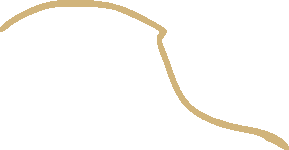
\includegraphics[width=0.32\linewidth]{chap_more/visu/filament__400.pdf}} 
	\subfloat{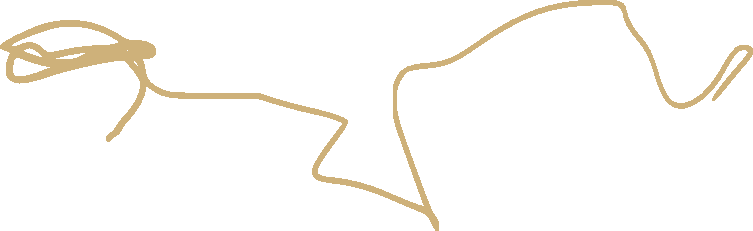
\includegraphics[width=0.32\linewidth]{chap_more/visu/filament__500.pdf}} 
	\subfloat{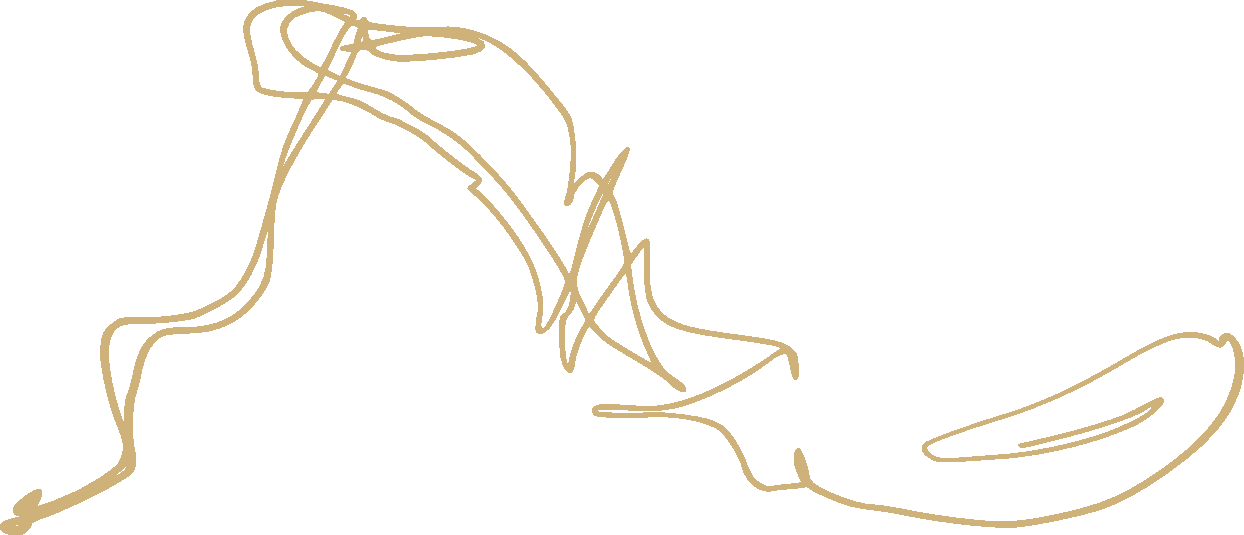
\includegraphics[width=0.32\linewidth]{chap_more/visu/filament__600.pdf}} 
	\caption{Filament visualisation for $t = 0.4 T_L$, $t = 0.5 T_L$ and $t = 0.6 T_L$}
	\label{fig:filament_stats}
\end{figure}
\begin{figure}
    \centering
    % Reynolds
\begin{tikzpicture}
	\begin{groupplot}[
			group style={
				group size=2 by 1,
				y descriptions at=edge left,
				%x descriptions at=edge bottom,
				horizontal sep=0.02\linewidth,
				vertical sep=0.02\linewidth,
			},
			% size
			width=0.5\textwidth,
			%height=0.33\textwidth,
			% y
			ylabel={$p(\varDelta)$},
			ymin=1e-3,
			ymax=1e5,
			ymode=log,
			% layers
			set layers,
			% legend
			legend columns=-1,
			legend cell align=left,
			legend style={draw=none, fill=none, at={(1.0, 1.05)}, anchor=south},
		]
	%\node[anchor=south east] at (1.4,4.3) {$t =$};
	\nextgroupplot[
		% x
		xlabel=$\varDelta_0/\KolmogorovScale$,
		xmin=0,
		xmax=1.0,
	]
		\addlegendimage{empty legend}\addlegendentry{$t = ~$}
		% plot
		\addplot
		[
		color=ColorSurf!100!ColorDuration,
		opacity=1.0,
		%only marks,%solid,
		mark=triangle*
		]
		table[
			x expr={\thisrowno{0} / 0.0028}, 
			y expr={\thisrowno{1}},
			col sep=comma, 
			comment chars=\#,
			unbounded coords=discard,
		]{app_dsm/data/filament/dobject__scalar_diff_pdf__d_0o0028__t_0o0.csv};
		\addlegendentry{0 \quad}
		% plot
		\addplot
		[
		color=ColorSurf!80!ColorDuration,
		opacity=1.0,
		%only marks,%solid,
		mark=square
		]
		table[
			x expr={\thisrowno{0} / 0.0028}, 
			y expr={\thisrowno{1}},
			col sep=comma, 
			comment chars=\#,
			unbounded coords=discard,
		]{app_dsm/data/filament/dobject__scalar_diff_pdf__d_0o0028__t_0o2.csv};
		\addlegendentry{0.1 $T_L$ \quad}
		% plot
		\addplot
		[
		color=ColorSurf!60!ColorDuration,
		opacity=1.0,
		%only marks,%solid,
		mark=pentagon*
		]
		table[
			x expr={\thisrowno{0} / 0.0028}, 
			y expr={\thisrowno{1}},
			col sep=comma, 
			comment chars=\#,
			unbounded coords=discard,
		]{app_dsm/data/filament/dobject__scalar_diff_pdf__d_0o0028__t_0o4.csv};
		\addlegendentry{0.2 $T_L$ \quad}
		% plot
		\addplot
		[
		color=ColorSurf!40!ColorDuration,
		opacity=1.0,
		%only marks,%solid,
		mark=o
		]
		table[
			x expr={\thisrowno{0} / 0.0028}, 
			y expr={\thisrowno{1}},
			col sep=comma, 
			comment chars=\#,
			unbounded coords=discard,
		]{app_dsm/data/filament/dobject__scalar_diff_pdf__d_0o0028__t_0o6.csv};
		\addlegendentry{0.3 $T_L$ \quad}
		% plot
		\addplot
		[
		color=ColorSurf!20!ColorDuration,
		opacity=1.0,
		%only marks,%solid,
		mark=*
		]
		table[
			x expr={\thisrowno{0} / 0.0028}, 
			y expr={\thisrowno{1}},
			col sep=comma, 
			comment chars=\#,
			unbounded coords=discard,
		]{app_dsm/data/filament/dobject__scalar_diff_pdf__d_0o0028__t_0o8.csv};
		\addlegendentry{0.4 $T_L$ \quad}
		% plot
		\addplot
		[
		color=ColorSurf!0!ColorDuration,
		opacity=1.0,
		%only marks,%solid,
		mark=star
		]
		table[
			x expr={\thisrowno{0} / 0.0028}, 
			y expr={\thisrowno{1}},
			col sep=comma, 
			comment chars=\#,
			unbounded coords=discard,
		]{app_dsm/data/filament/dobject__scalar_diff_pdf__d_0o0028__t_1o0.csv};
		\addlegendentry{0.5 $T_L$ \quad}
		% plot
		\addplot
		[
		color=ColorSurf!0!ColorDuration,
		opacity=1.0,
		%only marks,%solid,
		mark=diamond*
		]
		table[
			x expr={\thisrowno{0} / 0.0028}, 
			y expr={\thisrowno{1}},
			col sep=comma, 
			comment chars=\#,
			unbounded coords=discard,
		]{app_dsm/data/filament/dobject__scalar_diff_pdf__d_0o0028__t_1o2.csv};
		\addlegendentry{0.6 $T_L$ \quad}
	\nextgroupplot[
		% x
		xlabel=$\varDelta_s/\KolmogorovScale$,
		xmin=0,
		xmax=500,
	]
		\addplot[samples=2, black, dashed] coordinates {(1,1e-1)(1,1e5)};
		% plot
		\addplot
		[
		color=ColorSurf!100!ColorDuration,
		opacity=1.0,
		only marks,%solid,
		mark=triangle*,
		%mark options={scale=0.5},
		mark repeat=2,
		]
		table[
			x expr={\thisrowno{0} / 0.0028}, 
			y expr={\thisrowno{1}},
			col sep=comma, 
			comment chars=\#,
			unbounded coords=discard,
		]{app_dsm/data/filament/dobject__l_diff_pdf__d_0o0028__t_0o0.csv};
		% plot
		\addplot
		[
		color=ColorSurf!80!ColorDuration,
		opacity=1.0,
		only marks,%solid,
		mark=square,
		%mark options={scale=0.5},
		mark repeat=2,
		]
		table[
			x expr={\thisrowno{0} / 0.0028}, 
			y expr={\thisrowno{1}},
			col sep=comma, 
			comment chars=\#,
			unbounded coords=discard,
		]{app_dsm/data/filament/dobject__l_diff_pdf__d_0o0028__t_0o2.csv};
		% plot
		\addplot
		[
		color=ColorSurf!60!ColorDuration,
		opacity=1.0,
		only marks,%solid,
		mark=pentagon*,
		%mark options={scale=0.5},
		mark repeat=2,
		]
		table[
			x expr={\thisrowno{0} / 0.0028}, 
			y expr={\thisrowno{1}},
			col sep=comma, 
			comment chars=\#,
			unbounded coords=discard,
		]{app_dsm/data/filament/dobject__l_diff_pdf__d_0o0028__t_0o4.csv};
		% plot
		\addplot
		[
		color=ColorSurf!40!ColorDuration,
		opacity=1.0,
		only marks,%solid,
		mark=o,
		%mark options={scale=0.5},
		mark repeat=2,
		]
		table[
			x expr={\thisrowno{0} / 0.0028}, 
			y expr={\thisrowno{1}},
			col sep=comma, 
			comment chars=\#,
			unbounded coords=discard,
		]{app_dsm/data/filament/dobject__l_diff_pdf__d_0o0028__t_0o6.csv};
		% plot
		\addplot
		[
		color=ColorSurf!20!ColorDuration,
		opacity=1.0,
		only marks,%solid,
		mark=*,
		%mark options={scale=0.5},
		mark repeat=2,
		]
		table[
			x expr={\thisrowno{0} / 0.0028}, 
			y expr={\thisrowno{1}},
			col sep=comma, 
			comment chars=\#,
			unbounded coords=discard,
		]{app_dsm/data/filament/dobject__l_diff_pdf__d_0o0028__t_0o8.csv};
		% plot
		\addplot
		[
		color=ColorSurf!0!ColorDuration,
		opacity=1.0,
		only marks,%solid,
		mark=star,
		%mark options={scale=0.5},
		mark repeat=2,
		]
		table[
			x expr={\thisrowno{0} / 0.0028}, 
			y expr={\thisrowno{1}},
			col sep=comma, 
			comment chars=\#,
			unbounded coords=discard,
		]{app_dsm/data/filament/dobject__l_diff_pdf__d_0o0028__t_1o0.csv};
		% plot
		\addplot
		[
		color=ColorSurf!0!ColorDuration,
		opacity=1.0,
		only marks,%solid,
		mark=diamond*,
		%mark options={scale=0.5},
		mark repeat=2,
		]
		table[
			x expr={\thisrowno{0} / 0.0028}, 
			y expr={\thisrowno{1}},
			col sep=comma, 
			comment chars=\#,
			unbounded coords=discard,
		]{app_dsm/data/filament/dobject__l_diff_pdf__d_0o0028__t_1o2.csv};
	\end{groupplot}
\end{tikzpicture}

    \caption{
		Simulating a filament. Probability density function of the initial distance $\varDelta_0$ (left) and the curvilinear distance $\varDelta_s$ of pair of points spaced of a distance less than the Kolmogorov scale $\varDelta_{\vec{X}} < \KolmogorovScale$.
    }
    \label{fig:filament_stats}
\end{figure}
